\renewcommand{\thefootnote}{*}

\def\P{\mathcal P}
\def\ball#1{B_r ( #1 )}

\begin{frame}
\frametitle{Determining the shape from the gluing}

\begin{theorem}
	Each vertex of $\P$ lies within an $r$-ball centered at the corresponding \\
	vertex of $P$, where
	$r = E^2 \cdot  L \cdot 2 \sin ( \mathcal D \gamma / 2 ) + E \mu$.
\end{theorem} \vspace{-1.2mm}

\begin{figure}
	\centering
	\begin{subfigure}[m]{0.37\columnwidth}
		\centering
		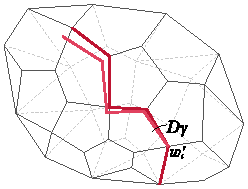
\includegraphics[scale=0.92]{figs_pres/anglePathOffset}
	\end{subfigure}
~
	\begin{subfigure}[m]{0.47\columnwidth}
		\centering
		\def\scopescale{0.45}
		\makecell[c]{\definecolor{ploskost}{RGB}{96,214,232}
\definecolor{sharik}{RGB}{181,56,43}

\def\flatn#1#2#3{(0.94868 * #1 cm + 0.4 * #2 cm,
	-0.31623 * #1 cm + 0.533333 * #2 cm + #3 cm)}
\def\punktir{\draw[dashed,color=hr]}
\def\thekrug#1{
	\filldraw #1 circle[radius=0.34mm];
	\filldraw[fill=sharik,fill opacity=0.72,draw=black] #1 circle [radius=0.5cm]}

\def\zleft{0.883883}
\def\zright{-1.767767}
\def\zz{-0.53033}

\def\pcenter{\flatn{-3}{0.5}{0}}
\def\ptangent{\flatn{-2.83333}{0.5}{0.471405}}

\def\qcenter{\flatn{0}{-2}{0}}
\def\qtangent{\flatn{-0.166667}{-2}{-0.471405}}

\def\rcenter{\flatn{0}{2}{0}}
\def\rtangent{\flatn{-0.166667}{2}{-0.471405}}

\def\sacenter{\flatn{2.5}{-0.5}{-2.3}}
\def\sbcenter{\flatn{2.5}{-0.5}{-0.65}}

\def\stransition{\flatn{2.5}{-0.5}{-1.41421}}
\def\sproj{\flatn{2.5}{-0.5}{0}}

\tikz{ \begin{scope}[scale=\scopescale]
% Кружок вершины p и то, что его обслуживает
	\punktir \ptangent -- \pcenter -- \flatn{-2.5}{0.5}{0};
	\punktir \pcenter -- \flatn{-3}{0}{0};
	\thekrug{\pcenter};
	\punktir \flatn{-2.5}{0.5}{0} -- \flatn{-1.5}{0.5}{0};
	\draw[thick] \flatn{-4}{0}{0} -- \flatn{-1.5}{0}{0};
%%

% Кружок вершины s_1 и то, что его обслуживает
	\punktir \flatn{2.5}{-0.5}{-1.8} -- \sacenter;
	\thekrug{\sacenter};
	\punktir \flatn{2.5}{-0.5}{-1.8} -- \stransition;
%%

% Та самая плоскость
	\filldraw[fill=ploskost,draw=ploskost, fill opacity=0.75]
		\flatn{-4}{3.075}{\zleft} -- \flatn{-4}{-3.075}{\zleft} --
		\flatn{3.5}{-3.075}{\zright} -- \flatn{3.5}{3.075}{\zright};
%%

% Несколько линий от точек касания
	\filldraw[fill=hr,draw=hr] \ptangent circle[radius=0.34mm];
	\punktir \ptangent -- \flatn{-1.5}{0.5}{0};
	\filldraw[fill=hr,draw=hr] \qtangent circle[radius=0.34mm];
	\punktir \qtangent -- \qcenter;
	\filldraw[fill=hr,draw=hr] \rtangent circle[radius=0.34mm];
	\punktir \rtangent -- \rcenter;
%%

% Кружок вершины s_2 и то, что его обслуживает
	\filldraw[fill=hr,draw=hr] \stransition circle[radius=0.34mm];
	\punktir \flatn{2.5}{-0.5}{-0.15} -- \stransition;
	\thekrug{\sbcenter};
	\punktir \flatn{2.5}{-0.5}{-0.15} -- \sproj;
	\punktir \flatn{0}{-0.5}{0} -- \sproj -- \flatn{2.5}{0}{0};
%%

% Два шарика на оси y
	\draw [thick,->] \flatn{0}{1.5}{0} -- \flatn{0}{3.75}{0};
	\thekrug{\rcenter};
	\draw [thick] \flatn{0}{-2.5}{0} -- \flatn{0}{1.5}{0};
	\thekrug{\qcenter};
	\draw [thick] \flatn{0}{-3.75}{0} -- \flatn{0}{-2.5}{0};
%%

% Линии, висящие в воздухе
	\punktir \flatn{-1.5}{0.5}{0} -- \flatn{0}{0.5}{0};
	\draw [thick,->] \flatn{-1.5}{0}{0} -- \flatn{4}{0}{0};
%%

% Подписи узлов
	\draw \pcenter node[left]{\footnotesize $p$};
	\draw \qcenter node[right]{\footnotesize\ \,$q$};
	\draw \rcenter node[right]{\footnotesize\ \ $r$};
	\draw \sacenter node[right]{\footnotesize $s_1$};
	\draw \sbcenter node[right]{\footnotesize\ \ $s_2$};
	\draw \stransition node[right]{\footnotesize $t$};
%%
\end{scope} }}
	\end{subfigure}
\end{figure} \vspace{-2.2mm}

This theorem allows to create a procedure for checking whether there is \\
a given edge in $\P$. The procedure was implemented.

\end{frame}